\begin{frame}
  \frametitle{Who am I\dots}

  \vspace{.5cm}

  \begin{flushleft}
    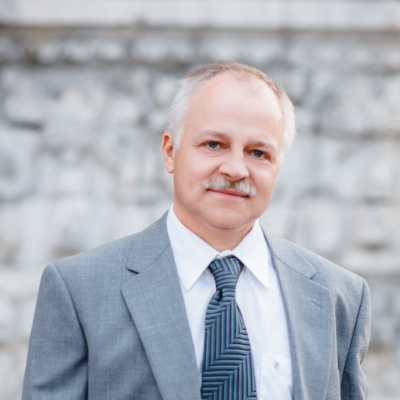
\includegraphics[height=3.5cm]{01-304_400_square.jpg}
  \end{flushleft}
  \vspace{-5cm}

  Embedded, modular, and real-time systems developer for almost 30 years

  \vspace{1cm}

  \begin{flushright}
    \begin{minipage}{10.5cm}

      \begin{itemize}
      \item i8051, i8080, i960, Digital Alpha, x86, MIPS, ARM, RISC-V
      \item CAMAC, VME, CompactPCI, AdvancedTCA, $\mu$TCA, SoMs
      \item FPGA and SoC-FPGA (Altera/Intel, Microsemi/Microchip)
      \end{itemize}
    \end{minipage}
  \end{flushright}

%  My usual problem with the software is how to make it run on a
%  hardware which is known not to be working yet and how to bring-up
%  and test this hardware. With a soft-core CPU it is getting even
%  worse.

\end{frame}
